\section{A sharp bound for rook substitutions}\label{sec:rook}

Let \(H=F_{74}\) have edges \(01,03,04,12,13,35,45\) on
\(\{0,\ldots,5\}\). Index the cells of a \(3\)-by-\(3\) board by
\((a,b)\in\{0,1,2\}^2\). In the graph \(R\), two cells are adjacent
when their row indices differ and their column indices differ. Thus \(R\)
is the complement of the rook graph. Figure~\ref{fig:rook} exhibits one
induced copy of \(H\) in \(R\). A finite \emph{rook substitution}
is either a single vertex or a substitution into \(R\) of nine nonempty
rook substitutions. The nine graphs may have different orders and depths.
Write \(R^k\) for the result when every branch has depth \(k\), with
\(R^0=K_1\) and \(|V(R^k)|=9^k\).

\begin{figure}[htb]
\centering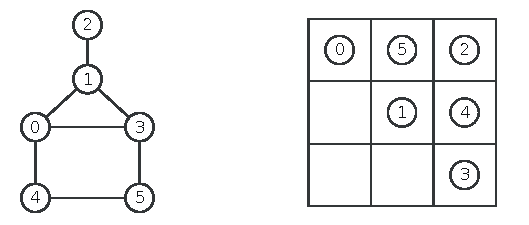
\includegraphics[width=.70\linewidth]{rook-example.pdf}
\caption{An induced copy of \(F_{74}\) in the nine-cell template.
Each vertex on the left occupies the cell with the same label on the
right. Two numbered cells are adjacent exactly when they lie in
different rows and different columns. The three blank cells are the
remaining vertices of the template.}
\label{fig:rook}
\end{figure}

\begin{theorem}\label{th:rook}
For a rook substitution \(G\) of order \(n\ge1\),
\[
 c_H(G)\le \frac{36(n^6-n)}{9^6-9}.
\]
Equality holds precisely for \(R^k\), \(k\ge0\). The largest limiting
density along these substitutions is \(D=360/7381\). For arbitrary
graphs the following rational bounds hold:
\[
 D\le\lambda_H\le
 U_R:=\frac{11321089900811290113624899}{232113757366008801543585792}.
\]
\end{theorem}

Row 74 of Table~3 of~\cite{six} gives \(0.0260416809\) as its lower
entry and \(0.0487738848\) as its numerical upper entry.
Here \(D=0.0487738788782\ldots\) and \(U_R-D<6.95\cdot10^{-9}\).
The rational upper bound is slightly larger than the published numerical
entry. It supplies an independently checkable endpoint.

Let \(\mathcal S\) be the six-subsets of the board inducing \(H\).
There are \(36\) such sets. This count takes only \(\binom96=84\)
tests: form the adjacency matrix on each set and compare it with the
permutations of the displayed edge list. A second finite test establishes
that \(H\) is prime: for each of its \(56\) subsets of sizes two through
five there is an outside vertex joined to some but not all of the subset.
Thus a copy meeting several children of a substitution uses six distinct
children.

\begin{lemma}\label{lem:rook}
For nonnegative cell masses \(x_0,\ldots,x_8\) of total mass one,
\[
 720\sum_{S\in\mathcal S}\prod_{v\in S}x_v
 \ \le\ D\left(1-\sum_{v=0}^{8}x_v^6\right).
\]
Equality holds at the uniform vector and at the nine vectors supported
on a single cell, and nowhere else.
\end{lemma}

\begin{proof}
We give the integer coefficient certificate. In an ordering \(\pi\) with
\(x_{\pi(0)}\le\cdots\le x_{\pi(8)}\), set
\(x_{\pi(j)}=d_0+\cdots+d_j\). All \(d_j\) are nonnegative.
Homogenise the proposed inequality and divide by \(D\). It suffices
to show that every coefficient of
\[
 \left(\sum_v x_v\right)^6-\sum_v x_v^6
       -14762\sum_{S\in\mathcal S}\prod_{v\in S}x_v
\]
is nonnegative in the variables \(d_j\), since \(720/D=14762\).
Index a monomial by a nondecreasing tuple \(t=(t_1,\ldots,t_6)\);
put \(m(t)=6!/\prod_j |\{i:t_i=j\}|!\).
The coefficient from the first two terms is
\[
 m(t)\left(\prod_{i=1}^6(9-t_i)-(9-t_6)\right).
\]
For the last sum, replace each cell of \(S\) by its rank in \(\pi\).
For each of the six ranks \(h\), choose an integer from \(0\) to \(h\).
Count the choices whose sorted list equals \(t\); sum these counts
over \(S\), and multiply by \(14762\).

Row permutations, column permutations and transposition give a group
of \(72\) board symmetries. Its action on the \(9!\) orderings is free.
The checker visits one ordering per orbit and performs the subtraction
just described for all \(\binom{14}6=3003\) monomials. All
\(5040\cdot3003=15\,135\,120\) differences are nonnegative. In every
ordering the coefficients of \(d_j^6\), \(1\le j\le7\), and of
\(d_0^4d_8^2\) are strictly positive. The full enumeration is specified
by the rank rule above and reproduced by the function
\texttt{rook} in the supplement.

At equality the seven intermediate increments vanish. The last positive
coefficient forces either \(d_8=0\) (all masses equal) or \(d_0=0\)
(one nonzero mass). Substitution gives equality in both cases, using
\(720\cdot36/(9^6-9)=D\).
\end{proof}

\begin{proof}[Proof of Theorem~\ref{th:rook}]
Let the child orders be \(n_0,\ldots,n_8\), with sum \(n\).
Primeness gives the exact count
\[
 c_H(G)=\sum_i c_H(G_i)+\sum_{S\in\mathcal S}\prod_{i\in S} n_i.
\]
Apply the lemma to \(n_i/n\), multiply by \(n^6/720\), and add the
inductive bounds for the children. The terms in \(\sum_i n_i^6\)
cancel, leaving \(D(n^6-n)/720\). Equality requires nine equal
positive orders and equality in every child. Induction from order one
then gives \(G=R^k\) up to isomorphism. Conversely these graphs attain
equality at every depth. Dividing by \(\binom n6\) and letting
\(n=9^k\) tend to infinity proves the limiting assertion.

For the unrestricted upper bound use the eight-vertex score \(s\) of
Section~\ref{sec:upper} with target \(H\), denominator \(2^{40}\), and the
169 integer factors in \texttt{f74/factors.txt}. These factors come
from the \href{https://github.com/bodnalev/supplementary_files/blob/9f356bb3dc10dcacd4d26a4eb1d556c2650e4e1b/graph_inducibility_6vtx/certs/inexact_74.pickle}{numerical certificate for \(F_{74}\)} of~\cite{six}.
For each of the \(12\,346\) eight-vertex hosts, the checker enumerates
its \(8!\) orderings, counts its induced copies of \(H\), and evaluates
the Gram terms. The largest integer numerator is
\(2377428879170370923861228790\) over \(8!\,2^{80}\); their ratio
reduces to \(U_R\). It occurs at host 10609 in the zero-based catalogue
order of the supplement. In particular, this score exceeds \(D\) by
\[
 U_R-D=\frac{11906124963772974494399}{1713231643118510964193206730752}.
\]
The orbit sizes sum to \(2^{28}\). Conditional
independence of the two flag extensions makes each Gram term
nonnegative in expectation, as in the proof of Theorem~\ref{th:global}.
Primeness of \(H\) again excludes repeated vertices in a sampled copy.
Taking the limit bounds \(\lambda_H\) by \(U_R\).
\end{proof}

To state the structural condition precisely, a graphon is a symmetric
measurable function \(W:[0,1]^2\to[0,1]\). Sample a graph by drawing
independent uniform points and, conditional on the points, placing
each edge independently with the probability given by \(W\).
The probability of obtaining \(H\) on \(h=|V(H)|\) points is \(p(H,W)\).
The graph limit theorem gives \(\lambda_H=\max_W p(H,W)\)~\cite{limits}.
Suppose a maximizer admits a measurable partition into nine
positive-measure cells with \(W\) equal almost everywhere on each
between-cell rectangle to the corresponding entry of the adjacency
matrix of \(R\). If the cell masses are \(x_i\)
and the unrestricted maximum is \(t\), the within-cell contributions
sum to at most \(t\sum_i x_i^6\). Lemma~\ref{lem:rook} bounds the rest
by \(D(1-\sum_i x_i^6)\). Then \(t\le D\), since \(\sum_i x_i^6<1\).
Thus a single maximizing graphon with such a partition would give the
unrestricted equality. The coefficient certificate proves the implication
under this partition hypothesis. The unconditional result proved here
is the interval in Theorem~\ref{th:rook}.

\section{A cycle and an isolated vertex}\label{sec:cycle}

Let \(J=F_{29}=C_5\sqcup K_1\). Conjecture~4.7 of~\cite{six} (v3)
gives the value \(24/1555\). Here \(C_5\) is the cycle on five vertices
and \(\sqcup\) denotes disjoint union. Write \(J[J]\) for the graph
obtained by substituting a copy of \(J\) at every vertex of \(J\).
We first give a counterexample whose
verification needs only a count of induced subgraphs of one finite graph.

\begin{theorem}\label{th:cycle}
The balanced independent blowup of the \(36\)-vertex graph \(J[J]\)
has limiting \(J\)-density \(12995/839808>24/1555\).
\end{theorem}

\begin{proof}
Index the six groups by the vertices of \(J\) and place a copy of \(J\)
in each. Between two groups put all edges if their indices are adjacent
in \(J\), and none otherwise. The cycle of an induced \(J\) must
lie in one group or use five distinct groups: \(C_5\) is prime, as is
seen by testing its subsets of sizes two through four.

In the latter case it occupies the five cycle groups. Each of these
is complete to two other occupied groups, so the isolated vertex must
lie in the sixth group. This gives \(6^6\) copies. If the cycle lies in
one group, that group contains exactly one induced \(C_5\). The isolated
vertex can lie in a different, nonadjacent group; there are \(20\)
ordered pairs of distinct nonadjacent groups and six choices of vertex
in the second. Finally, there is one entirely internal copy per group.
The total is \(6^6+20\cdot6+6=46\,782\).

Now replace each of the 36 vertices by an independent set of size \(m\).
Every pair of vertices in \(J\) has a third vertex distinguishing them,
so the six vertices of a copy occupy six different sets. Dividing
\(46\,782\,m^6\) by \(\binom{36m}6\) and passing to the limit gives
\[
 \frac{720\cdot46\,782}{36^6}=\frac{12995}{839808}
 =\frac{24}{1555}+\frac{51833}{1305901440}.
 \qedhere
\]
\end{proof}

A larger bound follows from two disconnected components. Let \(C\)
be the limit of iterated balanced substitutions into \(C_5\).
Equivalently, sample each point as an infinite word on five equiprobable
letters; the first letter at which two words differ determines their
adjacency in \(C_5\). Write \(c=p(C_5,C)\) and \(d=p(J,C)\).
For the cycle there are \(5!\) transversal assignments and five choices
for an entirely internal copy. For \(J\), a transversal cycle leaves
no group for an isolate. An internal cycle and an external isolate
use one of ten ordered nonadjacent pairs of groups; the isolate can
occupy any of the six sample positions. Hence
\[
 c=\frac{120+5c}{5^5}=\frac1{26},\qquad
 d=\frac{60c+5d}{5^6}=\frac3{20306}.
\]
Give two copies of \(C\) masses \(a=167216/10^6\) and \(b=1-a\)
and put no edges between them. The cycle stays in one component, while
the isolate may be in either. This gives the unrestricted lower bound
\begin{equation}\label{eq:cycles}
 \lambda_J\ge d(a^6+b^6)+6c(a^5b+ab^5)
 =\frac{722993599084786863008549024709}{46551227569580078125000000000000}.
\end{equation}
Finite-depth substitutions converge to these densities: the probability
that any two of six sampled words share a prefix of length \(k\) is
at most \(15/5^k\). Component sizes can be chosen in the given rational
ratio by uniform blowups.

\section{Three perturbations of recursive constructions}\label{sec:perturb}

Conjectures 4.5, 4.8 and 4.10 of~\cite{six} give rational values
for \(F_{22}, F_{34}\) and \(F_{62}\), respectively. The effect of changing
one mass parameter is small, so we give finite-depth witnesses and
take all comparisons in rational arithmetic.

\begin{theorem}\label{th:perturb}
\(\lambda_{F_{22}}>1440/23327\), and both
\(\lambda_{F_{34}}\) and \(\lambda_{F_{62}}\) exceed \(5760/88573\).
Each strict inequality already holds for the limiting density of a
blowup of the two-level pattern defined below.
\end{theorem}

Use the graphs and templates in Table~\ref{tab:parts}. A listed pair
of distinct parts is complete, and every other such pair is empty.
A part marked recursive receives a scaled copy of the whole construction.
Of the remaining parts all are independent for \(F_{22}\) and \(F_{34}\),
and all are cliques for \(F_{62}\). These specifications use the edge
lists in the \emph{statements} of the three conjectures in v3.

\begin{table}[htb]
\centering\small
\begin{tabular}{@{}llll@{}}
\toprule
Graph & Edges of the target & Edges between parts & Recursive parts\\
\midrule
\(F_{22}\) & 01 03 04 12 15 & 01 02 13 & 0, 1\\
\(F_{34}\) & 01 02 03 04 12 15 & 01 02 03 04 14 23 24 25 45 & 0, 2, 4\\
\(F_{62}\) & 01 03 04 05 12 13 45 & 01 05 12 14 15 23 24 25 35 & 1, 2, 5\\
\bottomrule
\end{tabular}
\caption{Templates for the perturbations. Part labels start at zero.}
\label{tab:parts}
\end{table}

Let \(r\) count the recursive parts. There are also \(r\) constant parts.
Give each recursive part mass \(x\) and each constant part mass
\(y=1/r-x\), for \(0<x<1/r\).

\begin{proof}
The contribution from six points in at least two parts is
\(A_r(x)=c_r x^2y^4\), with \(c_2=180\) and \(c_3=2160\).
Here is an explicit enumeration for these coefficients. Fix the
labelling of the target in Table~\ref{tab:parts}. Run over the
\((2r)^6\) maps from its vertices to the parts, omitting constant maps.
Discard a map if some required edge or nonedge disagrees with a fixed
bit of the template. In each surviving map exactly two target vertices
use recursive parts and they use different parts. Thus every required
bit is already determined. Multiply the number of surviving maps by
the number of distinct labellings of the target, \(6!/|\Aut(F)|\).
In table order there are \(2,6,6\) surviving maps and \(90,360,360\)
labellings, giving \(180,2160,2160\).
These finite counts are repeated in the supplement by assigning one
vertex at a time and pruning on the first conflicting pair.

Let \(q=rx^6\). Six points in one constant part cannot give any of the
three targets. Six points in one recursive part restart the count.
After two levels, finish all remaining recursive parts by independent
sets. The resulting density is
\[
 B_r(x)=A_r(x)(1+q).
\]
There are \(2r^2+r\) terminal parts. For rational masses this density
is attained in the limit of finite graphs by taking part sizes in those
proportions. Sampling six vertices without replacement and sampling
six independent part labels have the same limit.

For completeness, the infinite recursion has density
\(D_r(x)=A_r(x)/(1-q)\). At \(x_0=1/(3r)\) its values are exactly
the respective conjectured fractions. On \(0<x<1/r\), its derivative
has the sign of \(1-3rx+2rx^6\), which is positive at \(x_0\).
To certify the finite-depth claim, substitute the following rational
choices directly in \(B_r\). The final column gives strict lower
bounds on the difference, with the entries interpreted as exact rationals.
\[
\begin{array}{c c c c}
 r & x & D_r(x_0) & B_r(x)-D_r(x_0)\\
 2 & 166681/10^6 & 1440/23327 & >5/10^{10}\\
 3 & 111112/10^6 & 5760/88573 & >9/10^{12}
\end{array}
\]
Both inequalities follow by clearing the positive denominators. The
supplement also flattens the two levels into a single matrix and
recounts compatible assignments directly with the terminal masses.
\end{proof}
